\scanpage{77}
\mspage{6}
now every actual path $x\longrightarrow y$ (given by a continuous map $[0,1]\longrightarrow X$) decomposes into \inserted{a composite of} \inserted{``direct''} paths
\diagram{\begin{tikzcd}[ampersand replacement=\&,column sep=small]
x_0=x \arrow[r] \& x_1 \arrow[r] \& x_2\,\mathord{-}\,\mathord{-} \arrow[r] \& x_n=y
\end{tikzcd}}
between ``nearby'' \deleted{paths} \inserted{points}. In the \deleted{general} case \inserted{where the $X_\alpha$ are closed}, a descent argument (as already noted in the first hypothesis) gives the stated result.

This second proof has the advantage of also working to \inserted{show} the somewhat more general result, and perhaps more interesting from the practical point of view, where for every $\alpha$ one has $I_\alpha\subset T_\alpha$ a \inserted{nonempty} subset of $T_\alpha$ (normally, a finite subset) in such a way that for $T_\alpha\subset T_\beta$ one has $I_\alpha\subset I_\beta$ \unsure{and|,} (normally, one first takes a suitable $I\subset X_K$ and takes $I_\alpha=I\cap T_\alpha$, hence $I=\bigcup I_\alpha$), and one restricts oneself to the $g^\alpha_{y,x}$ for $x,y\in I_\alpha$: knowledge of them makes it possible to recover \uline{all} \inserted{$f_l(u)$,} $g_{\deleted{\unsure{yx}}l}(u)$, $l$ an arbitrary path in

\margin{One has two ways of ``recovering'' the action of $\Gamma$ on the groupoid $\widehat{\Pi}_1(X,I)$ (where $I\subset X_K$) in some sense dual to one another: either one takes a system of generators $l_j:x_j\mathbin{-}y_j$ $(x_j,y_j\in I)$ for $\Pi_1(X,I)$, and looks at the $f_{l_j}(u)$ or $g_{l_j}(u)$, or one fixes some $T_\alpha$ as above, and one looks at the $g^\alpha_{x,y}$ $(\alpha\in A,x,y\in T_\alpha\cap I)$. In fact one very soon sees that it is \deleted{\unsure{ff}} unnecessary to suppose that the $T_\alpha$ cover $X$ (for example if the $T_\alpha$ are the supports of the paths $l_j$).}

\figure{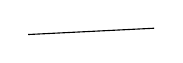
\begin{tikzpicture}\draw (0,0)--(1.6,.08);\end{tikzpicture}}
Up to now, we have kept $X$, $u$ fixed, we have varied $l$, resp. $(T/X,x,y)$. If we look at what happens for variable $u\in\Gamma$, the formulas
\margin{76}
